%卒論発表会は発表12分、質問3分です。



\documentclass[dvipdfmx,cjk]{beamer}
\bibliographystyle{junsrt}

% 各種色の設定
% 自分で好きな色を定義して使うことができる(colorパッケージが必要?)
% 以下の例だと、berryという色が使えるようになる
\definecolor{berry}{RGB}{234,97,142}
\definecolor{usuhanada}{RGB}{80,126,164}


% プリアンブル
% Beamerに必要なパッケージ
\usepackage{graphicx}
\usepackage{hyperref}
\usepackage{fancybox}
\usepackage{pgfpages}

% その他、普段使うもの(必要に応じて追加)
\usepackage{ascmac}
\usepackage{color}
\usepackage{amsmath}
\usepackage{fancybox}
\usepackage{moreverb}
\usepackage{latexsym}
\usepackage{amsthm}
\usepackage{proof}
\usepackage{stmaryrd}
\usepackage{amssymb}
\usepackage{marvosym}
\usepackage{verbatim}
\usepackage{setspace}
\usepackage{smartdiagram}
\usepackage[ipaex]{pxchfon}
\usepackage{graphics}
\usepackage{tikz}
\usepackage[ipaex]{pxchfon}
\usepackage[dvipdfmx]{graphicx}

\definecolor{ikkonzome}{rgb}	{	0.9961	,	0.7569	,	0.7373	}
\definecolor{ishitake}{rgb}	{	0.9961	,	0.6941	,	0.7059	}
\definecolor{momo}{rgb}	        {	0.9961	,	0.6824	,	0.8039	}
\definecolor{kobai}{rgb}	{	0.9412	,	0.4235	,	0.5569	}
\definecolor{nakabeni}{rgb}	{	0.9451	,	0.2706	,	0.4941	}
\definecolor{sakura}{rgb}	{	0.9333	,	0.8353	,	0.8353	}
\definecolor{arazome}{rgb}	{	0.9725	,	0.7216	,	0.7843	}
\definecolor{usubeni}{rgb}	{	0.8471	,	0.4471	,	0.5451	}
\definecolor{hisame}{rgb}	{	0.7451	,	0.4039	,	0.4039	}
\definecolor{toki}{rgb}	        {	0.9569	,	0.6431	,	0.6353	}
\definecolor{sakuranezumi}{rgb}	{	0.6941	,	0.6039	,	0.6078	}
\definecolor{sango}	{rgb}	{	0.8471	,	0.4157	,	0.3725	}
\definecolor{akane}	{rgb}	{	0.7529	,	0.0118	,	0.3451	}
\definecolor{choshun}{rgb}	{	0.7490	,	0.5255	,	0.5255	}
\definecolor{karakurenai}{rgb}	{	0.7373	,	0.0118	,	0.2667	}
\definecolor{enji}{rgb}	        {	0.6275	,	0.0863	,	0.3176	}
\definecolor{keshiaka}{rgb}	{	0.6275	,	0.4275	,	0.4275	}
\definecolor{kokiake}{rgb}	{	0.5059	,	0.0706	,	0.2549	}
\definecolor{jinzamomi}{rgb}	{	0.9098	,	0.4549	,	0.4157	}
\definecolor{mizugaki}{rgb}	{	0.7294	,	0.5529	,	0.4784	}
\definecolor{umenezumi}{rgb}	{	0.5882	,	0.3922	,	0.3882	}
\definecolor{suoko}{rgb}        {	0.5843	,	0.2667	,	0.2431	}
\definecolor{akabeni}{rgb}	{	0.8039	,	0.0784	,	0.3725	}
\definecolor{shinshu}{rgb}	{	0.6431	,	0.0353	,	0.0000	}
\definecolor{azuki}{rgb}	{	0.5255	,	0.0235	,	0.0000	}
\definecolor{ginshu}{rgb}	{	0.7490	,	0.2824	,	0.0588	}
\definecolor{ebicha}{rgb}	{	0.4549	,	0.2706	,	0.2627	}
\definecolor{kuriume}{rgb}	{	0.5843	,	0.3804	,	0.4314	}
\definecolor{akebono}{rgb}	{	0.8902	,	0.5961	,	0.4941	}
\definecolor{hanezu}{rgb}	{	0.7882	,	0.5961	,	0.5373	}
\definecolor{sangoshu}{rgb}	{	0.8196	,	0.5059	,	0.4471	}
\definecolor{shozyohi}{rgb}	{	0.7686	,	0.0000	,	0.0000	}
\definecolor{shikancha}{rgb}	{	0.5569	,	0.3294	,	0.1882	}
\definecolor{kakishibu}{rgb}	{	0.6745	,	0.4078	,	0.3333	}
\definecolor{benikaba}{rgb}	{	0.7137	,	0.3373	,	0.2941	}
\definecolor{benitobi}{rgb}	{	0.6196	,	0.3176	,	0.2706	}
\definecolor{benihihada}{rgb}	{	0.5020	,	0.3137	,	0.2353	}
\definecolor{kurotobi}{rgb}	{	0.3176	,	0.2000	,	0.1490	}
\definecolor{benihi}{rgb}	{	0.8235	,	0.4745	,	0.1922	}
\definecolor{terigaki}{rgb}	{	0.8118	,	0.4627	,	0.1804	}
\definecolor{ake}{rgb}	        {	0.7804	,	0.3098	,	0.1725	}
\definecolor{edocha}{rgb}	{	0.6863	,	0.4353	,	0.2941	}
\definecolor{bengara}{rgb}	{	0.6392	,	0.1569	,	0.0196	}
\definecolor{hihada}{rgb}	{	0.5412	,	0.3412	,	0.2353	}
\definecolor{shishi}{rgb}	{	0.8549	,	0.6863	,	0.5961	}
\definecolor{araishu}{rgb}	{	0.9294	,	0.4902	,	0.4549	}
\definecolor{akago}{rgb}	{	0.8118	,	0.5765	,	0.4275	}
\definecolor{tokigaracha}{rgb}	{	0.7922	,	0.5255	,	0.3686	}
\definecolor{otan}{rgb}	        {	0.8157	,	0.4157	,	0.2235	}
\definecolor{komugi}{rgb}	{	0.8157	,	0.6549	,	0.5098	}
\definecolor{rakuda}{rgb}	{	0.6784	,	0.5255	,	0.4118	}
\definecolor{tsurubami}{rgb}	{	0.6275	,	0.4392	,	0.3961	}
\definecolor{ama}{rgb}	        {	0.7765	,	0.6902	,	0.5843	}
\definecolor{nikkei}{rgb}	{	0.7216	,	0.4667	,	0.3725	}
\definecolor{renga}{rgb}	{	0.6902	,	0.3765	,	0.3098	}
\definecolor{sohi}{rgb}   	{	0.8078	,	0.5098	,	0.2078	}
\definecolor{enshucha}{rgb}	{	0.6706	,	0.4275	,	0.1608	}
\definecolor{karacha}{rgb}	{	0.5765	,	0.4235	,	0.1490	}
\definecolor{kabacha}{rgb}	{	0.6353	,	0.3725	,	0.1569	}
\definecolor{sodenkaracha}{rgb}	{	0.5216	,	0.3490	,	0.1373	}
\definecolor{suzumecha}{rgb}	{	0.4745	,	0.3176	,	0.1255	}
\definecolor{kurikawacha}{rgb}	{	0.4078	,	0.2745	,	0.1098	}
\definecolor{momoshiocha}{rgb}	{	0.3490	,	0.2353	,	0.0902	}
\definecolor{tobi}{rgb}	        {	0.4353	,	0.3098	,	0.1412	}
\definecolor{kurumizome}{rgb}	{	0.6667	,	0.5333	,	0.3333	}
\definecolor{kaba}{rgb}	        {	0.8196	,	0.4588	,	0.1294	}
\definecolor{korosen}{rgb}	{	0.5059	,	0.3843	,	0.1608	}
\definecolor{kogecha}{rgb}	{	0.3333	,	0.2549	,	0.1098	}
\definecolor{kokikuchinashi}{rgb}	{	0.8078	,	0.5922	,	0.3490	}
\definecolor{araigaki}{rgb}	{	0.8157	,	0.5529	,	0.3176	}
\definecolor{taisha}{rgb}	{	0.6353	,	0.4196	,	0.2078	}
\definecolor{akashirotsurubami}{rgb}	{	0.8078	,	0.6118	,	0.4157	}
\definecolor{tonocha}{rgb}	{	0.5922	,	0.4039	,	0.2000	}
\definecolor{sencha}{rgb}	{	0.5255	,	0.3529	,	0.1490	}
\definecolor{sharegaki}{rgb}	{	0.8549	,	0.7098	,	0.4863	}
\definecolor{ko}{rgb}	        {	0.9529	,	0.8275	,	0.6627	}
\definecolor{usugaki}{rgb}	{	0.8627	,	0.7294	,	0.5294	}
\definecolor{koji}{rgb}	        {	0.8275	,	0.6039	,	0.2706	}
\definecolor{umezome}{rgb}	{	0.8667	,	0.7373	,	0.4235	}
\definecolor{beniukon}{rgb}	{	0.8549	,	0.5843	,	0.2549	}
\definecolor{chojicha}{rgb}	{	0.5569	,	0.4000	,	0.1098	}
\definecolor{kenpozome}{rgb}	{	0.3059	,	0.2667	,	0.0627	}
\definecolor{biwacha}{rgb}	{	0.7333	,	0.5294	,	0.1922	}
\definecolor{kohaku}{rgb}	{	0.8039	,	0.5961	,	0.2471	}
\definecolor{usuko}{rgb}	{	0.8745	,	0.7373	,	0.4824	}
\definecolor{kuchiba}{rgb}	{	0.8157	,	0.6157	,	0.3216	}
\definecolor{kincha}{rgb}	{	0.7725	,	0.4902	,	0.2000	}
\definecolor{chozizome}{rgb}	{	0.5686	,	0.3961	,	0.1608	}
\definecolor{kitsune}{rgb}	{	0.6392	,	0.4431	,	0.1804	}
\definecolor{hushizome}{rgb}	{	0.5804	,	0.4353	,	0.1608	}
\definecolor{kyara}{rgb}	{	0.4510	,	0.3373	,	0.1255	}
\definecolor{susutake}{rgb}	{	0.4588	,	0.3529	,	0.1176	}
\definecolor{shirocha}{rgb}	{	0.7529	,	0.6588	,	0.4118	}
\definecolor{odo}{rgb}	        {	0.7137	,	0.6039	,	0.3137	}
\definecolor{ginsusutake}{rgb}	{	0.5608	,	0.4745	,	0.2392	}
\definecolor{kigaracha}{rgb}	{	0.7490	,	0.6196	,	0.2745	}
\definecolor{kobicha}	{rgb}	{	0.5020	,	0.4118	,	0.1765	}
\definecolor{usuki}	{rgb}	{	0.8549	,	0.7804	,	0.4275	}
\definecolor{yamabuki}	{rgb}	{	0.9098	,	0.8000	,	0.2039	}
\definecolor{tamago}	{rgb}	{	0.8275	,	0.7412	,	0.3373	}
\definecolor{hajizome}	{rgb}	{	0.7412	,	0.6039	,	0.2431	}
\definecolor{yamabukicha}{rgb}	{	0.7059	,	0.5765	,	0.2275	}
\definecolor{kuwazome}	{rgb}	{	0.6471	,	0.5255	,	0.2118	}
\definecolor{namakabe}	{rgb}	{	0.5569	,	0.4549	,	0.1843	}
\definecolor{kuchinashi}{rgb}	{	0.8078	,	0.7333	,	0.3843	}
\definecolor{tomorokoshi}{rgb}	{	0.7804	,	0.7020	,	0.2941	}
\definecolor{shirotsurubami}{rgb}	{	0.8745	,	0.8235	,	0.5922	}
\definecolor{kitsurubami}{rgb}	{	0.6863	,	0.6039	,	0.2118	}
\definecolor{toou}	{rgb}	{	0.8353	,	0.7725	,	0.4235	}
\definecolor{hanaba}	{rgb}	{	0.8549	,	0.8000	,	0.4941	}
\definecolor{torinoko}	{rgb}	{	0.8431	,	0.8118	,	0.6902	}
\definecolor{ukon}	{rgb}	{	0.8039	,	0.7216	,	0.3059	}
\definecolor{kikuchiba}	{rgb}	{	0.7765	,	0.6667	,	0.2902	}
\definecolor{rikyushiracha}{rgb}{	0.6627	,	0.6471	,	0.4784	}
\definecolor{rikyucha}	{rgb}	{	0.5176	,	0.5176	,	0.2588	}
\definecolor{aku}	{rgb}	{	0.5294	,	0.5059	,	0.4039	}
\definecolor{higosusutake}{rgb}	{	0.4863	,	0.4510	,	0.3059	}
\definecolor{rokocha}	{rgb}	{	0.4157	,	0.4353	,	0.3686	}
\definecolor{mirucha}	{rgb}	{	0.4471	,	0.4471	,	0.3725	}
\definecolor{natane}	{rgb}	{	0.7216	,	0.6863	,	0.3882	}
\definecolor{kimirucha}	{rgb}	{	0.5373	,	0.5059	,	0.2549	}
\definecolor{uguisucha}	{rgb}	{	0.4118	,	0.3882	,	0.1961	}
\definecolor{nanohana}	{rgb}	{	0.9882	,	0.9882	,	0.3804	}
\definecolor{kariyasu}	{rgb}	{	0.8039	,	0.7686	,	0.3882	}
\definecolor{kihada}	{rgb}	{	0.9608	,	0.9137	,	0.2863	}
\definecolor{zoge}	{rgb}	{	0.8863	,	0.8235	,	0.7216	}
\definecolor{wara}	{rgb}	{	0.7882	,	0.7490	,	0.4706	}
\definecolor{macha}	{rgb}	{	0.6235	,	0.6392	,	0.4863	}
\definecolor{yamabato}	{rgb}	{	0.5137	,	0.5176	,	0.4000	}
\definecolor{mushikuri}	{rgb}	{	0.8196	,	0.8000	,	0.6118	}
\definecolor{aokuchiba}	{rgb}	{	0.6275	,	0.6392	,	0.3451	}
\definecolor{hiwacha}	{rgb}	{	0.6784	,	0.6863	,	0.4196	}
\definecolor{ominaeshi}	{rgb}	{	0.8745	,	0.8863	,	0.4039	}
\definecolor{wasabi}	{rgb}	{	0.5922	,	0.6824	,	0.5765	}
\definecolor{uguisu}	{rgb}	{	0.3333	,	0.4118	,	0.0627	}
\definecolor{hiwa}	{rgb}	{	0.7098	,	0.7216	,	0.2392	}
\definecolor{aoshirotsurubami}{rgb}	{	0.5961	,	0.6471	,	0.4471	}
\definecolor{yanagicha}	{rgb}	{	0.5373	,	0.5725	,	0.3529	}
\definecolor{rikancha}	{rgb}	{	0.3333	,	0.4196	,	0.2863	}
\definecolor{aikobicha}	{rgb}	{	0.2706	,	0.3412	,	0.2353	}
\definecolor{koke}	{rgb}	{	0.4941	,	0.5686	,	0.3922	}
\definecolor{miru}	{rgb}	{	0.1529	,	0.3216	,	0.1843	}
\definecolor{sensai}	{rgb}	{	0.1373	,	0.2863	,	0.1608	}
\definecolor{baiko}	{rgb}	{	0.5529	,	0.6157	,	0.3922	}
\definecolor{iwai}	{rgb}	{	0.3059	,	0.4118	,	0.2784	}
\definecolor{hiwamoegi}	{rgb}	{	0.4431	,	0.6824	,	0.2431	}
\definecolor{yanagisusutake}{rgb}	{	0.2039	,	0.3333	,	0.1255	}
\definecolor{urayanagi}	{rgb}	{	0.5843	,	0.6824	,	0.2431	}
\definecolor{usumoegi}	{rgb}	{	0.4824	,	0.6706	,	0.2275	}
\definecolor{yanagizome}{rgb}	{	0.4353	,	0.6000	,	0.2078	}
\definecolor{moegi}	{rgb}	{	0.3020	,	0.5961	,	0.1882	}
\definecolor{aoni}	{rgb}	{	0.1216	,	0.4196	,	0.2431	}
\definecolor{matsuba}	{rgb}	{	0.1098	,	0.3686	,	0.2118	}
\definecolor{usuao}	{rgb}	{	0.5529	,	0.7059	,	0.6118	}
\definecolor{wakatake}	{rgb}	{	0.3843	,	0.6824	,	0.5059	}
\definecolor{yanaginezumi}{rgb}	{	0.5020	,	0.6078	,	0.5490	}
\definecolor{oitake}	{rgb}	{	0.4157	,	0.5412	,	0.4392	}
\definecolor{sensaimidori}{rgb}	{	0.2549	,	0.3882	,	0.2627	}
\definecolor{midori}	{rgb}	{	0.0000	,	0.4824	,	0.0000	}
\definecolor{byakuroku}	{rgb}	{	0.6078	,	0.7333	,	0.6196	}
\definecolor{sabiseiji}	{rgb}	{	0.5333	,	0.6588	,	0.5804	}
\definecolor{rokusho}	{rgb}	{	0.3373	,	0.6039	,	0.4039	}
\definecolor{tokusa}	{rgb}	{	0.2549	,	0.4706	,	0.3922	}
\definecolor{onandocha}	{rgb}	{	0.2039	,	0.3725	,	0.3098	}
\definecolor{aotake}	{rgb}	{	0.1412	,	0.5176	,	0.4353	}
\definecolor{rikyunezumi}{rgb}	{	0.4157	,	0.5686	,	0.5490	}
\definecolor{birodo}	{rgb}	{	0.1059	,	0.4275	,	0.3608	}
\definecolor{mishiao}	{rgb}	{	0.1098	,	0.4588	,	0.3882	}
\definecolor{aimirucha}	{rgb}	{	0.2510	,	0.4000	,	0.3608	}
\definecolor{tonotya}	{rgb}	{	0.3059	,	0.4941	,	0.4392	}
\definecolor{mizuasagi}	{rgb}	{	0.1569	,	0.6745	,	0.6745	}
\definecolor{seji}	{rgb}	{	0.4745	,	0.6588	,	0.5922	}
\definecolor{seheki}	{rgb}	{	0.0588	,	0.5569	,	0.4824	}
\definecolor{sabitetsu}	{rgb}	{	0.0392	,	0.3294	,	0.2784	}
\definecolor{tetsu}	{rgb}	{	0.0627	,	0.3961	,	0.3961	}
\definecolor{omeshicha}	{rgb}	{	0.0667	,	0.4667	,	0.4667	}
\definecolor{korainando}{rgb}	{	0.0588	,	0.3922	,	0.0392	}
\definecolor{minatonezumi}{rgb}	{	0.4549	,	0.6000	,	0.6118	}
\definecolor{aonibi}	{rgb}	{	0.1804	,	0.3725	,	0.3882	}
\definecolor{tetsuonando}{rgb}	{	0.1961	,	0.4118	,	0.4275	}
\definecolor{mizu}	{rgb}	{	0.5451	,	0.7412	,	0.7608	}
\definecolor{sabiasagi}	{rgb}	{	0.4510	,	0.6000	,	0.6000	}
\definecolor{kamenozoki}{rgb}	{	0.7098	,	0.9020	,	0.8902	}
\definecolor{asagi}	{rgb}	{	0.3020	,	0.6784	,	0.7098	}
\definecolor{shinbashi}	{rgb}	{	0.0000	,	0.6000	,	0.6353	}
\definecolor{sabionando}{rgb}	{	0.2392	,	0.3961	,	0.3843	}
\definecolor{ainezumi}	{rgb}	{	0.2235	,	0.4000	,	0.3843	}
\definecolor{ai}	{rgb}	{	0.2039	,	0.3765	,	0.4314	}
\definecolor{onando}	{rgb}	{	0.1843	,	0.3686	,	0.4000	}
\definecolor{hanaasagi}	{rgb}	{	0.2000	,	0.6196	,	0.7098	}
\definecolor{chigusa}	{rgb}	{	0.1922	,	0.5725	,	0.6745	}
\definecolor{masuhana}	{rgb}	{	0.1569	,	0.4667	,	0.5569	}
\definecolor{hanada}	{rgb}	{	0.0039	,	0.4275	,	0.5373	}
\definecolor{noshimehana}{rgb}	{	0.1412	,	0.4235	,	0.5098	}
\definecolor{omeshionando}{rgb}	{	0.1176	,	0.3529	,	0.4235	}
\definecolor{sora}	{rgb}	{	0.1451	,	0.7216	,	0.8039	}
\definecolor{konpeki}	{rgb}	{	0.0902	,	0.5098	,	0.7333	}
\definecolor{kurotsurubami}{rgb}{	0.0627	,	0.3137	,	0.3451	}
\definecolor{gunjo}	{rgb}	{	0.5098	,	0.7882	,	0.9098	}
\definecolor{kon}	{rgb}	{	0.0000	,	0.2000	,	0.4000	}
\definecolor{kachi}	{rgb}	{	0.0000	,	0.1765	,	0.3490	}
\definecolor{ruri}	{rgb}	{	0.0078	,	0.3922	,	0.6510	}
\definecolor{konjo}	{rgb}	{	0.0039	,	0.3137	,	0.5216	}
\definecolor{rurikon}	{rgb}	{	0.0000	,	0.3020	,	0.5020	}
\definecolor{benimidori}{rgb}	{	0.3373	,	0.4588	,	0.6784	}
\definecolor{konkikyo}	{rgb}	{	0.0039	,	0.0667	,	0.4275	}
\definecolor{hujinezumi}{rgb}	{	0.3216	,	0.3686	,	0.6118	}
\definecolor{benikakehana}{rgb}	{	0.2275	,	0.2471	,	0.5882	}
\definecolor{hujiiro}	{rgb}	{	0.4706	,	0.4863	,	0.7059	}
\definecolor{hutaai}	{rgb}	{	0.3137	,	0.3333	,	0.5608	}
\definecolor{hujimurasaki}{rgb}	{	0.4157	,	0.3333	,	0.5686	}
\definecolor{kikyo}	{rgb}	{	0.3529	,	0.3216	,	0.5725	}
\definecolor{shion}	{rgb}	{	0.5137	,	0.4196	,	0.6784	}
\definecolor{messhi}	{rgb}	{	0.2196	,	0.1765	,	0.3098	}
\definecolor{shikon}	{rgb}	{	0.2510	,	0.1961	,	0.3529	}
\definecolor{kokimurasaki}{rgb}	{	0.3098	,	0.2000	,	0.3765	}
\definecolor{usu}	{rgb}	{	0.7294	,	0.6353	,	0.7843	}
\definecolor{hashita}	{rgb}	{	0.6000	,	0.4549	,	0.6706	}
\definecolor{rindo}	{rgb}	{	0.5922	,	0.5137	,	0.7529	}
\definecolor{sumire}	{rgb}	{	0.3882	,	0.2157	,	0.5922	}
\definecolor{nasukon}	{rgb}	{	0.3216	,	0.2235	,	0.4353	}
\definecolor{murasaki}	{rgb}	{	0.3137	,	0.1765	,	0.4824	}
\definecolor{kurobeni}	{rgb}	{	0.2353	,	0.1294	,	0.3059	}
\definecolor{ayame}	{rgb}	{	0.4275	,	0.1569	,	0.5098	}
\definecolor{benihuji}	{rgb}	{	0.6824	,	0.5333	,	0.6667	}
\definecolor{edomurasaki}{rgb}	{	0.3961	,	0.1529	,	0.4392	}
\definecolor{kodaimurasaki}{rgb}{	0.4353	,	0.2863	,	0.4627	}
\definecolor{shikon}{rgb}       {	0.4118	,	0.2549	,	0.3765	}
\definecolor{hatobanezumi}{rgb}	{	0.4235	,	0.3804	,	0.4392	}
\definecolor{budonezumi}{rgb}	{	0.3412	,	0.2196	,	0.3529	}
\definecolor{ebizome}	{rgb}	{	0.4000	,	0.2235	,	0.3882	}
\definecolor{hujisusutake}{rgb}	{	0.2549	,	0.0824	,	0.2471	}
\definecolor{usuebi}	{rgb}	{	0.6549	,	0.4392	,	0.6039	}
\definecolor{botan}	{rgb}	{	0.6706	,	0.0392	,	0.4353	}
\definecolor{umemurasaki}{rgb}	{	0.6667	,	0.3922	,	0.5176	}
\definecolor{nisemurasaki}{rgb}	{	0.3686	,	0.0000	,	0.3216	}
\definecolor{murasakitobi}{rgb}	{	0.3922	,	0.3255	,	0.3529	}
\definecolor{ususuo}{rgb}	{	0.7569	,	0.4000	,	0.5412	}
\definecolor{suo}{rgb}	        {	0.6941	,	0.0627	,	0.4157	}
\definecolor{kuwanomi}{rgb}	{	0.4196	,	0.0549	,	0.2745	}
\definecolor{nibi}{rgb}	        {	0.4549	,	0.4235	,	0.3961	}
\definecolor{benikeshi}{rgb}	{	0.4118	,	0.3804	,	0.3843	}
\definecolor{shironeri}{rgb}	{	0.9843	,	0.9843	,	0.9843	}
\definecolor{shironezumi}{rgb}	{	0.6471	,	0.6588	,	0.6627	}
\definecolor{ginnezumi}{rgb}	{	0.5255	,	0.5490	,	0.5922	}
\definecolor{sunezumi}{rgb}	{	0.4275	,	0.4392	,	0.4392	}
\definecolor{dobunezumi}{rgb}	{	0.2863	,	0.2941	,	0.2941	}
\definecolor{aisumicha}{rgb}	{	0.2078	,	0.2196	,	0.2510	}
\definecolor{binrojizome}{rgb}	{	0.2118	,	0.0824	,	0.0706	}
\definecolor{sumizome}{rgb}	{	0.2706	,	0.2706	,	0.2706	}





% Beamerの設定
% スタイル
\usetheme{Berlin}%Szeged} %Darmstadt %Berlin
% フォント
\usefonttheme{professionalfonts}
% 色
\usecolortheme[RGB={80,126,164}]{structure}
% タイトルのフォント
\setbeamerfont{title}{size=\Large, series=\bfseries}
% フレームタイトルのフォント
\setbeamerfont{frametitle}{size=\Large, series=\bfseries}
% 日本語用の設定(多分)
\renewcommand{\familydefault}{\sfdefault}
\renewcommand{\kanjifamilydefault}{\gtdefault}
\mathversion{bold}

\newenvironment{slide}[1][]{\begin{frame}\frametitle{#1}}{\end{frame}}

\newcommand{\freebox}[2][1.0]{\scalebox{#1}{\ensuremath{#2}}}
\newcommand{\leftfunctor}[2]{#1^{\triangleright}#2}
\newcommand{\rightfunctor}[2]{#1^{\triangleleft}#2}
\newcommand{\formula}[2]{\textbf{#1} & \begin{array}[t]{l} #2 \end{array}}

% スライド番号
\setbeamertemplate{footline}[frame number]
\setbeamerfont{footline}{size=\small,series=\bfseries}
\setbeamercolor{footline}{fg=usuhanada,bg=usuhanada}

% Sectionが変わるごとに目次が出るようにしたいときは以下を追加
%\AtBeginSection[]{
%    \begin{frame}
%        \tableofcontents[currentsection]
%    \end{frame}
%}

% 参考文献の引用をテキスト表示
\setbeamertemplate{bibliography item}[text]
\setbeamercolor{bibliography entry author}{fg=black,bg=white}
\setbeamercolor{bibliography entry journal}{fg=black,bg=white}


% ナビゲーションシンボルを消す
\setbeamertemplate{navigation symbols}{}

% Adobeの目次の文字化け解消
\usepackage{atbegshi}
\ifnum 42146=\euc"A4A2 \AtBeginShipoutFirst{\special{pdf:tounicode EUC-UCS2}}\else
\AtBeginShipoutFirst{\special{pdf:tounicode 90ms-RKSJ-UCS2}}\fi

%appendixでページ番号を出さない
\newcommand{\backupbegin}{
   \newcounter{framenumberappendix}
   \setcounter{framenumberappendix}{\value{framenumber}}
}
\newcommand{\backupend}{
   \addtocounter{framenumberappendix}{-\value{framenumber}}
   \addtocounter{framenumber}{\value{framenumberappendix}}
}



\title{RNN変換モデル用いた高階論理からの文生成}
\subject{卒業研究発表会}
\author[]{馬目 華奈}
\institute{戸次研究室}
\date{
卒業研究発表会\\
February 6, 2018}



% 本体
\begin{document}

% \begin{frame}〜\end{frame}まででスライド1枚
\begin{frame}
  \titlepage
\end{frame}

% 目次
%\begin{frame}[]{もくじ}
% \tableofcontents
% もくじ
%\end{frame}

%%%%%%%%%%%%%%%%%%%%%%%%
\begin{frame}
\frametitle{研究背景}
\begin{center}
\begin{figure}[h]
	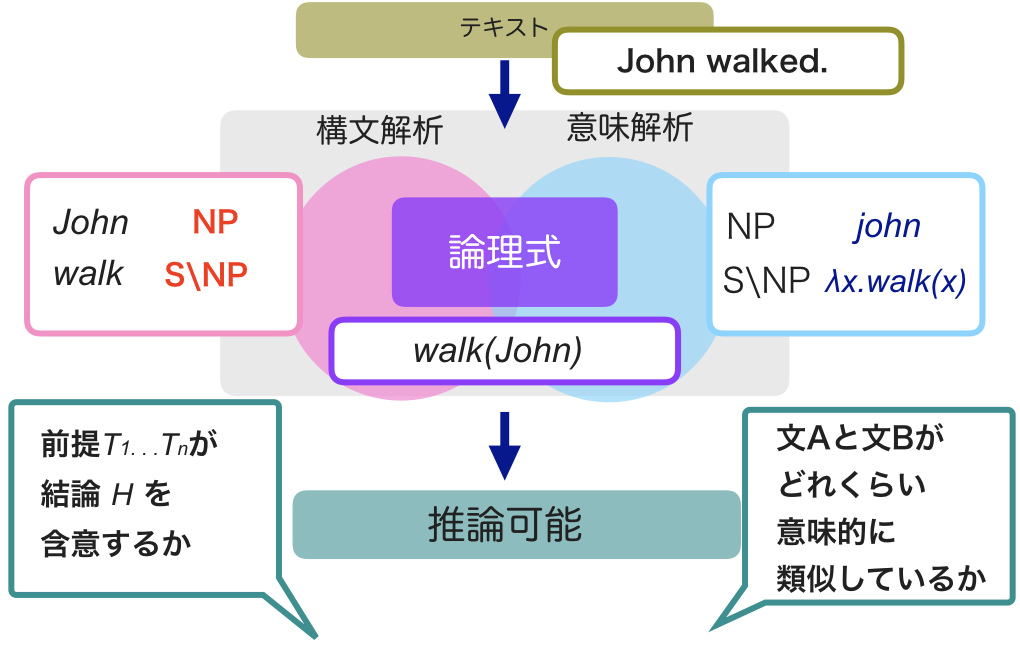
\includegraphics[width=10cm]{backend1.png}
        \label{fig:backend1}
\end{figure}
\end{center}

%\begin{itemize}
% \item 近年の構文解析と意味解析の技術の発展によって,文の意味を論理式で表して高度な推論を行うシステムの構築が可能となった.
% \item このようなシステムは,含意関係認識や文間類似度計算のタスクで高精度 を達成しており,今後,さらなる自然言語処理タスクへの応用が期待されている.
% \item 文からその論理式への変換が高精度に行われる一方で,論理式を自然言語文に戻す方法については自明ではない.
% \item 論理式から自然言語文に逆変換する ことができれば,推論システムの改善や,様々な自然 言語処理タスクへの応用が期待できる.
%\end{itemize}

%文字色を変えたいときは、{\color{berry} こう。}
\end{frame}
%%%%%%%%%%%%%%%%%%%%%%%%%


%%%%%%%%%%%%%%%%%%%%%%%%
\begin{frame}
\frametitle{研究背景}
\begin{center}
\begin{figure}[h]
	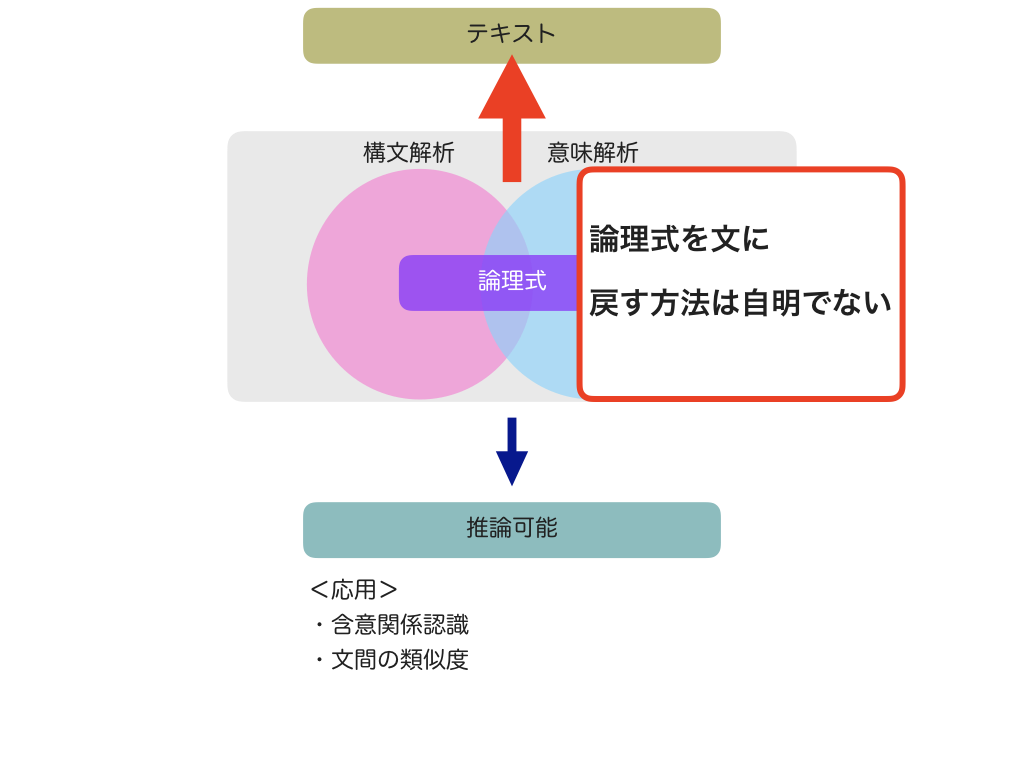
\includegraphics[width=10cm]{backend2.png}
        \label{fig:backend2}
\end{figure}
\end{center}
\end{frame}
%%%%%%%%%%%%%%%%%%%%%%%%%

%%%%%%%%%%%%%%%%%%%%%%%%
\begin{frame}
\frametitle{研究背景}
\begin{center}
\begin{figure}[h]
	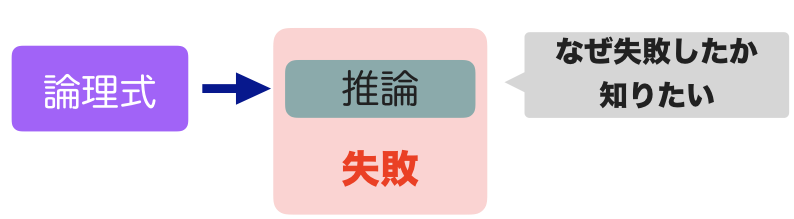
\includegraphics[width=8cm]{backend4.png}
        \label{fig:backend4}
\end{figure}
\end{center}
\begin{block}{前提が足りない例}
  \begin{itemize}
    \item All women ordered coffee or tea.
    \item Some woman ordered tea.
  \end{itemize}
\end{block}
\begin{block}{知識が足りない例}
  \begin{itemize}
    \item All women ordered drink.
    \item Some woman ordered tea.
  \end{itemize}
\end{block}

\end{frame}
%%%%%%%%%%%%%%%%%%%%%%%%%



%%%%%%%%%%%%%%%%%%%%%%%%%
\begin{frame}
\frametitle{研究概要}
\begin{center}
  \smartdiagramset{back arrow disabled=true}
  \smartdiagram[flow diagram:horizontal]{高階論理式,embedding,系列変換モデル,文}
\end{center}
\begin{block}{}
  \begin{itemize}
    \item ニューラルネットによる系列変換モデルを用いて\\高階論理式から文を生成する手法を提案.
    \item 埋め込みの際,4種の手法\\(記号,トークン,木構造,グラフ)を検討する.
  \end{itemize}
\end{block}

\end{frame}
%%%%%%%%%%%%%%%%%%%%%%%%%


%%%%%%%%%%%%%%%%%%%%%%%%%
\begin{frame}
\frametitle{関連研究1}
\begin{center}
  \smartdiagramset{back arrow disabled=true, set color list={toki,gray,gray,gray},}
  \smartdiagram[flow diagram:horizontal]{高階論理式,embedding,系列変換モデル,文}
\end{center}
\begin{block}{}
  \begin{itemize}
    \item ニューラルネットによる系列変換モデルを用いて\\{\color{berry}高階論理式}から文を生成する手法を提案.
    \item 埋め込みの際,4種の手法\\(記号,トークン,木構造,グラフ)を検討する.
  \end{itemize}
\end{block}

\end{frame}
%%%%%%%%%%%%%%%%%%%%%%%%%


%%%%%%%%%%%%%%%%%%%%%%%%%
\begin{frame}
\frametitle{関連研究:CCG に基づく論理式による文の意味表現}
\begin{center}
\begin{figure}[h]
	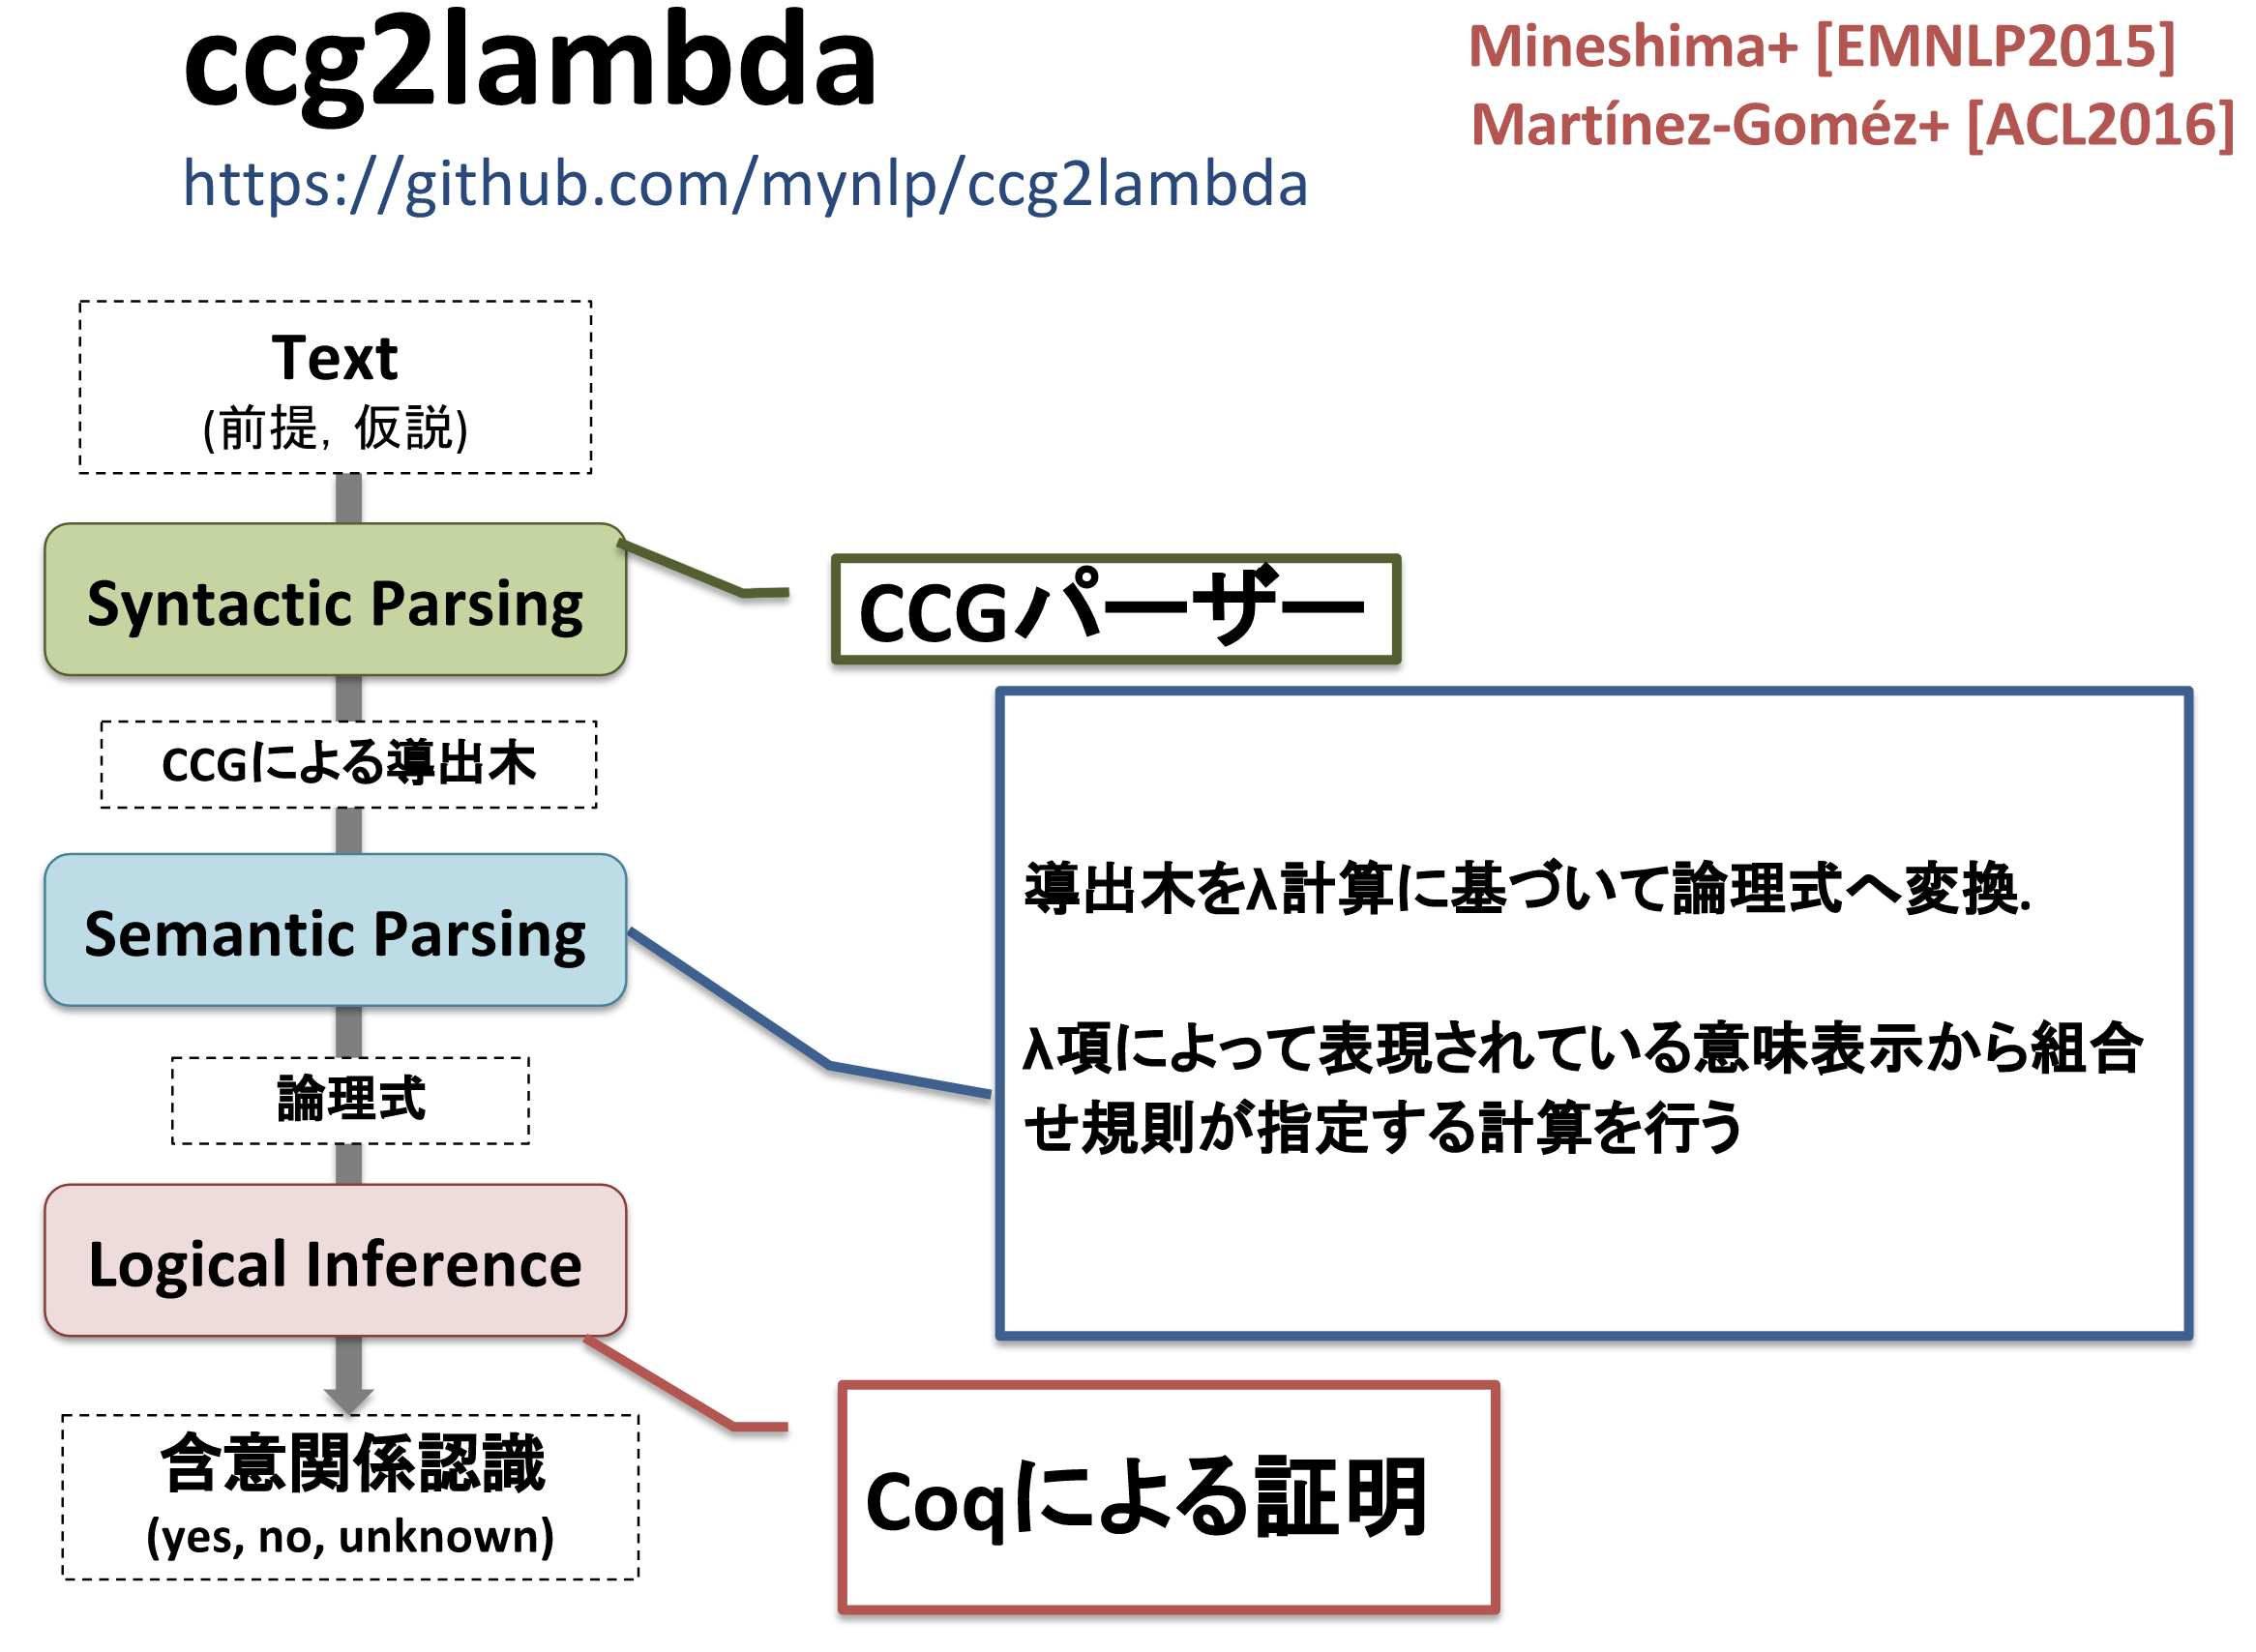
\includegraphics[width=10cm]{c2l.png}
        \label{fig:c2l}
\end{figure}
\end{center}

\end{frame}
%%%%%%%%%%%%%%%%%%%%%%%%%



%%%%%%%%%%%%%%%%%%%%%%%%%
%\begin{frame}
%\frametitle{関連研究:意味表現からの文生成}
%\end{frame}
%%%%%%%%%%%%%%%%%%%%%%%%%

%%%%%%%%%%%%%%%%%%%%%%%%%
\begin{frame}
\frametitle{関連研究2}
\begin{center}
  \smartdiagramset{back arrow disabled=true, set color list={gray,gray,shion,gray},}
  \smartdiagram[flow diagram:horizontal]{高階論理式,embedding,系列変換モデル,文}
\end{center}
\begin{block}{}
  \begin{itemize}
    \item {\color{berry}ニューラルネットによる系列変換モデル}を用いて高階論理式から文を生成する手法を提案.\cite{seq2seq}
    \item 埋め込みの際,4種の手法\\(記号,トークン,木構造,グラフ)を検討する.
  \end{itemize}
\end{block}

\end{frame}
%%%%%%%%%%%%%%%%%%%%%%%%%



%%%%%%%%%%%%%%%%%%%%%%%%%
\begin{frame}
\frametitle{関連研究:系列変換モデル }
\begin{itemize}
  \item 入出力がシーケンスとなるニューラルネットのモデル
  \item エンコータ:入力列を再帰型NNにより隠れ状態ベクトルに変換
  \item デコーダ:隠れ状態ベクトルを初期値とし,\\隠れ状態と自身のこれまでの出力結果を基に\\次のトークンを生成
\end{itemize}

\begin{center}
\begin{figure}[h]
	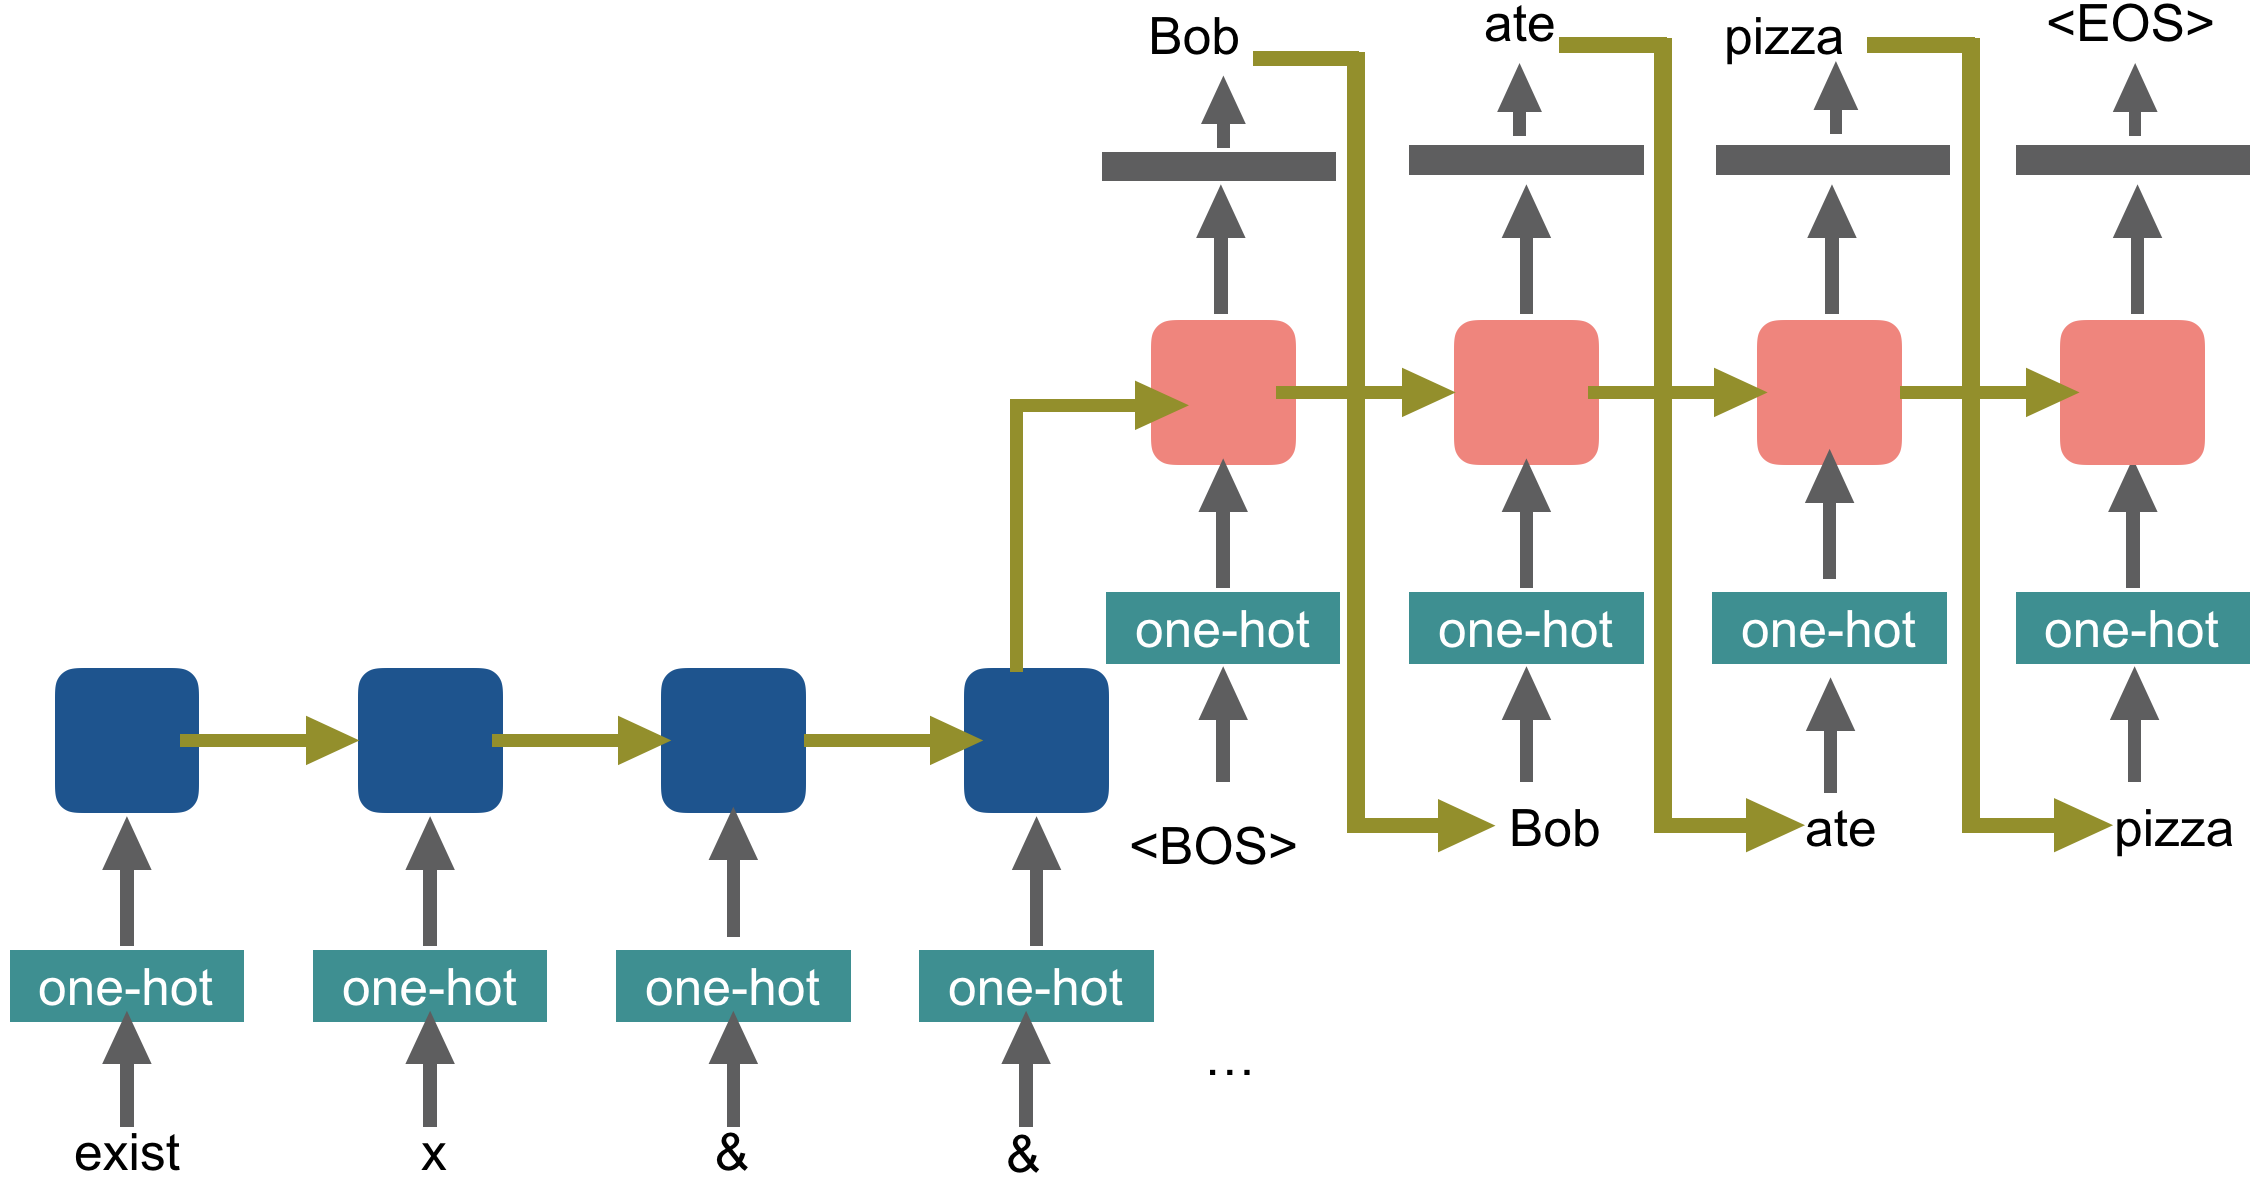
\includegraphics[width=8cm]{learn_model.png}
        \label{fig:seq2seq}
\end{figure}
\end{center}

\end{frame}
%%%%%%%%%%%%%%%%%%%%%%%%%

%%%%%%%%%%%%%%%%%%%%%%%%%
\begin{frame}
\frametitle{提案手法}
\begin{center}
  \smartdiagramset{back arrow disabled=true, set color list={gray,mizuasagi,gray,gray},}
  \smartdiagram[flow diagram:horizontal]{高階論理式,embedding,系列変換モデル,文}
\end{center}
\begin{block}{}
  \begin{itemize}
    \item ニューラルネットによる系列変換モデルを用いて\\高階論理式から文を生成する手法を提案.
    \item 埋め込みの際,4種の手法\\{\color{berry}(記号,トークン,木構造,グラフ)}を検討する.
  \end{itemize}
\end{block}

\end{frame}
%%%%%%%%%%%%%%%%%%%%%%%%%


%%%%%%%%%%%%%%%%%%%%%%%%%
\begin{frame}
\frametitle{提案手法:論理式埋め込み1}
例:exists x.((x = Bob)\&exists z1.(Pizza(z1)\& exists e.(eat(e) \& (Subj(e) = x) \& (Obj(e) = z1) )))
\begin{block}{記号ごとに区切る}
  スペース,カッコを込みで埋め込む
  [e,x,i,s,t,s, ,x, ,., ,(,(,x, ,=,...]
\end{block}
\begin{block}{トークンごとに区切る}
  トークンごとなのでスペースを除くことができるが,カッコは入る.
  [exists,x,(,(,x,=,Bob,exists,z1,...]
\end{block}
\end{frame}
%%%%%%%%%%%%%%%%%%%%%%%%%


%%%%%%%%%%%%%%%%%%%%%%%%%
\begin{frame}
\frametitle{提案手法:論理式埋め込み2}
\begin{columns}[t]
    \begin{column}{0.5\textwidth} % 左:60%
      \begin{block}{記号ごとに区切る}
        \begin{figure}[h]
        \begin{center}
        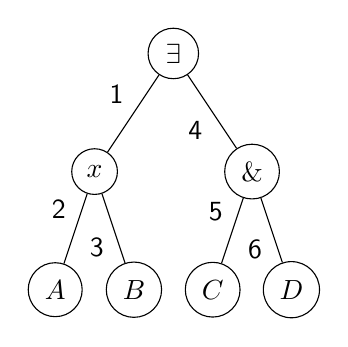
\begin{tikzpicture}[
          level 1/.style={sibling distance=20mm},
          level 2/.style={sibling distance=10mm},
          nodeop/.style={circle,draw}
        ]
        \node[nodeop]  {$\exists$}
          child { node[nodeop] {$x$}
            child { node[nodeop] {$A$} edge from parent node [auto,swap]{2} }
            child { node[nodeop] {$B$} edge from parent node [auto,swap]{3}}
            edge from parent node [auto,swap]{1}
          }
          child { node[nodeop]  {$\&$}
            child { node[nodeop]  {$C$} edge from parent node [auto,swap]{5}}
            child { node[nodeop]  {$D$} edge from parent node [auto,swap]{6}}
            edge from parent node [auto,swap]{4}
          };
        \end{tikzpicture}
        \end{center}
        \end{figure}
      \end{block}
    \end{column}
    \begin{column}{0.5\textwidth} % 右:40%
      \begin{block}{}
        \begin{itemize}
          \item 論理式をポーランド記法に変換する\\(論理演算子を前にもってくる)
          \item pre-orderでたどる
          \item $[exists,x,\&,=,x,Bob,exists,z1,...]$
        \end{itemize}
      \end{block}
    \end{column}
\end{columns}

\end{frame}
%%%%%%%%%%%%%%%%%%%%%%%%%



%%%%%%%%%%%%%%%%%%%%%%%%%
\begin{frame}
\frametitle{提案手法:論理式埋め込み3}
\begin{columns}[t]
    \begin{column}{0.5\textwidth} % 左:60%
      \begin{block}{グラフ}
        \begin{figure}[h]
        	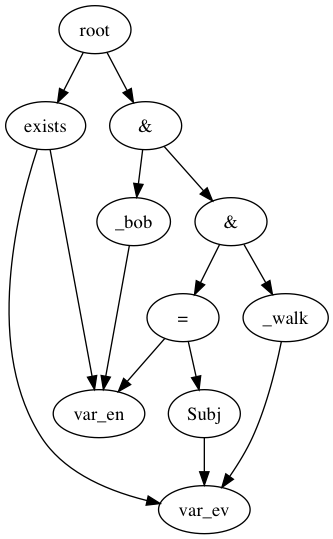
\includegraphics[width=4cm]{graph.png}
                \label{fig:graph}
        \end{figure}
      \end{block}
    \end{column}
    \begin{column}{0.5\textwidth} % 右:40%
      \begin{block}{}
        \begin{itemize}
          \item $[exists,<var\_en>,<var\_en>,...]$
        \end{itemize}
      \end{block}
    \end{column}
\end{columns}

\end{frame}
%%%%%%%%%%%%%%%%%%%%%%%%%




%%%%%%%%%%%%%%%%%%%%%%%%%
%\begin{frame}
%\frametitle{提案手法:学習モデル}
%\end{frame}
%%%%%%%%%%%%%%%%%%%%%%%%%

%%%%%%%%%%%%%%%%%%%%%%%%%
\begin{frame}
\frametitle{提案手法:データセット}
\begin{itemize}
  \item
SNLIを用い論理式と文のペアを作成

\item 60単語以内の文例を対象
train:9140/dev:2285/test:1500\\

\end{itemize}
\begin{center}
\begin{figure}[h]
	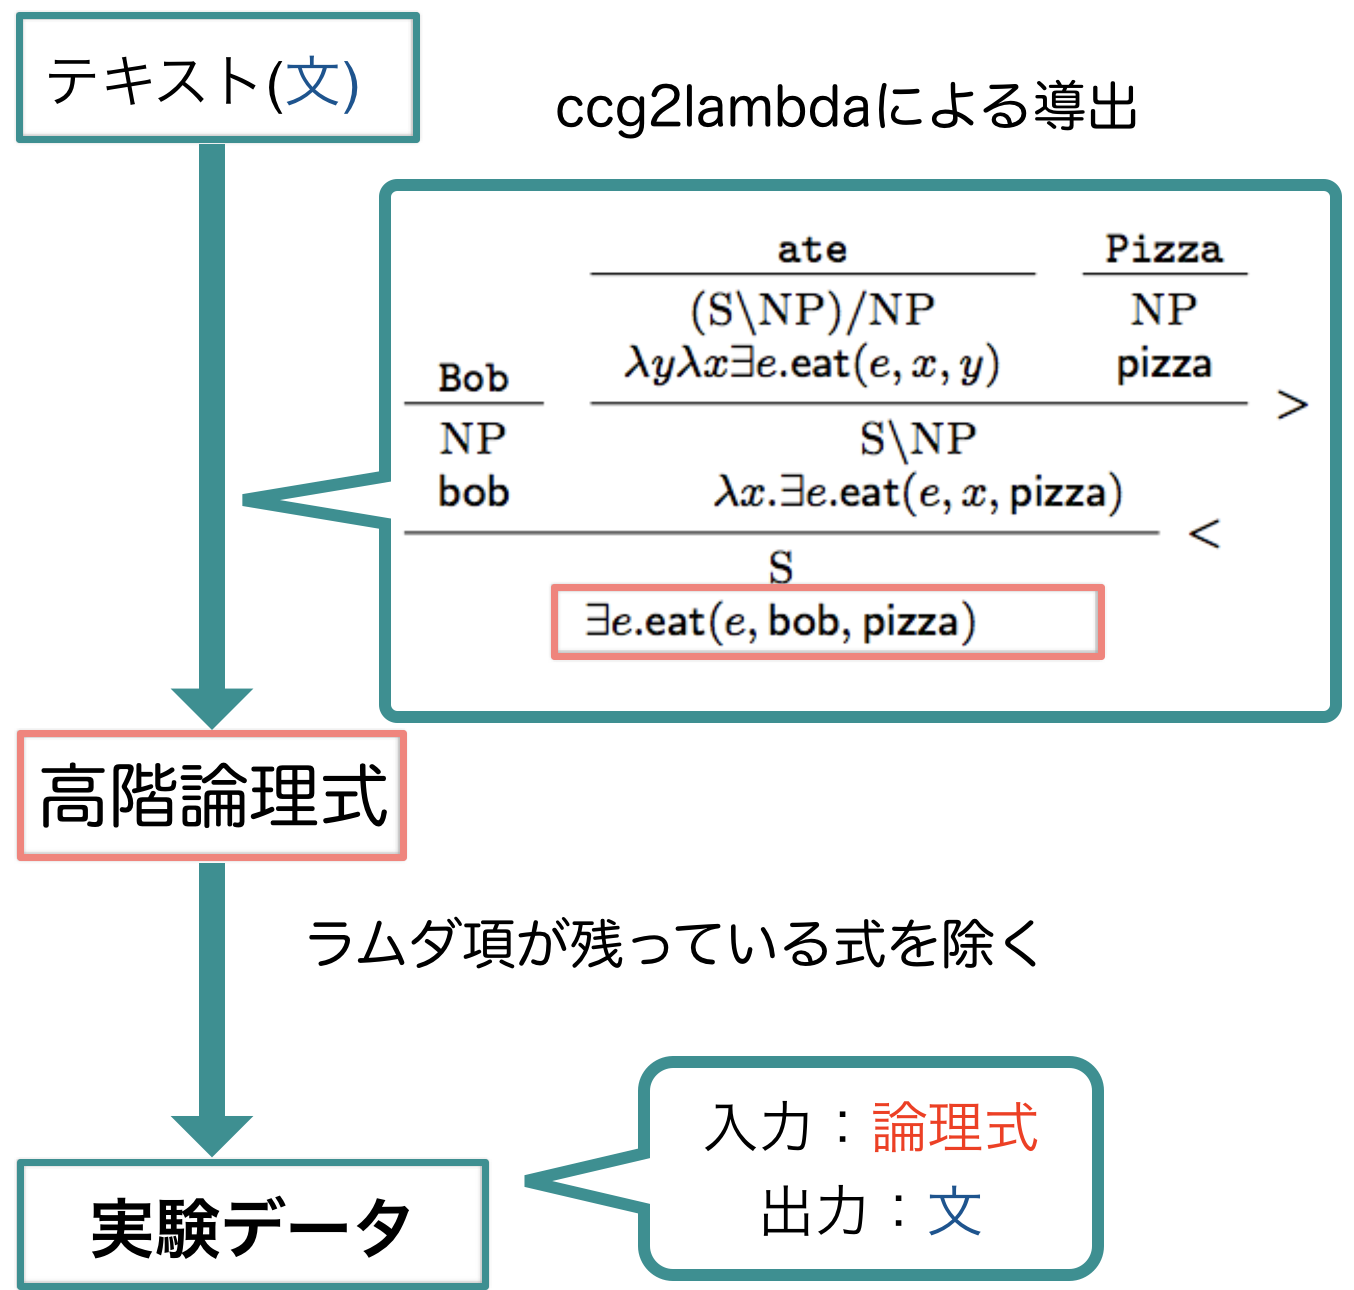
\includegraphics[width=6cm]{edit_data.png}
        \label{fig:editdata}
\end{figure}
\end{center}

\end{frame}
%%%%%%%%%%%%%%%%%%%%%%%%%

%%%%%%%%%%%%%%%%%%%%%%%%%
\begin{frame}
\frametitle{実験:実験設定}

\begin{itemize}
\item 系列変換モデルによる文生成 (入力:論理式,出力:文)
\item トークンベースのLSTMの出力次元数をLSTMの出力次元数を256
\end{itemize}

\begin{center}
  \begin{tabular}{rrrrr}
    \hline
       & 記号 & トークン & 木構造 & グラフ \\
    \hline \hline
    入力語彙数  & 70  &  5,118 & 5,107 & 4,991\\
    出力語彙数  & 78   & 7,214 & 7,214 & 7,214\\
    入力列最長 & 2,097  & 699 & 451 & 259 \\
    出力列最長 & 270  & 55 & 53 & 53 \\
    \hline
  \end{tabular}
\end{center}

\begin{block}{環境,ライブラリ}
\begin{itemize}
\item tsubameサーバ(メモリ240GiB,GPU× 4)
\item ニューラルネットのモデル:Keras
\item logic関係:nltk
\end{itemize}
\end{block}

\end{frame}
%%%%%%%%%%%%%%%%%%%%%%%%%

%%%%%%%%%%%%%%%%%%%%%%%%%
\begin{frame}
\frametitle{実験:評価方法}
\begin{block}{BLEUによる評価}
%\begin{figure}[h]
%	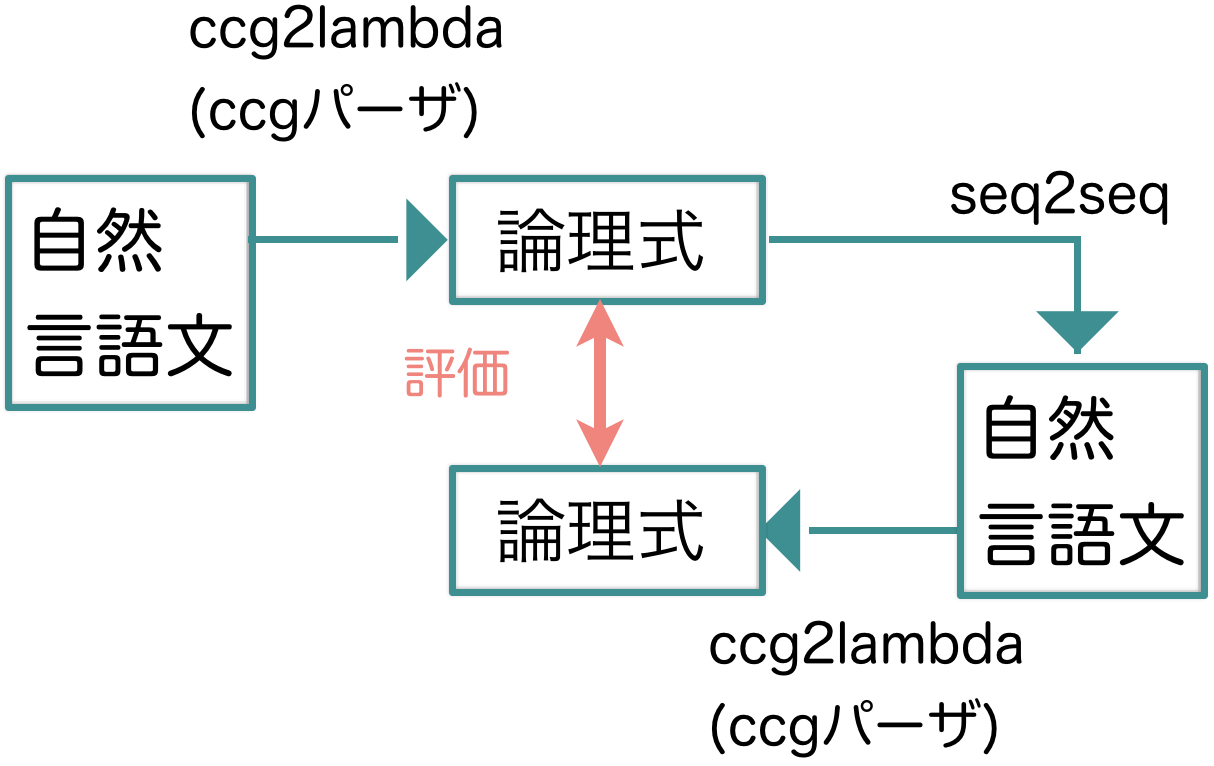
\includegraphics[width=6cm]{eval.png}
%        \label{fig:eval}
%\end{figure}

\[
	\mathit{score} = \mathit{BP}\exp\left(\sum_{i=1}^N \frac{1}{N}\log P_n\right)
\]
\[
  \mathit{BP} = \left\{ \begin{array}{ll}
    1 &  (c \geq r) \\
    \exp\left(1- \frac{r}{c}\right) & ($c $ < $ r$)
  \end{array} \right.
\]
\\
\[
	P_n = \frac{\sum_{i=0}\text{出力文i中と解答文i中で一致した}n\mathchar`-gram\text{数}}{\sum_{i=0}\text{出力文i中の全}n\mathchar`-gram\text{数}}
\]

\end{block}


\end{frame}
%%%%%%%%%%%%%%%%%%%%%%%%%

%%%%%%%%%%%%%%%%%%%%%%%%%
\begin{frame}
\frametitle{実験:実験結果}
\begin{block}{BLEU評価}
  \label{table:evaluation}
  \centering
  \begin{tabular}{ccccc}
    \hline
    指標  & 記号 & トークン & 木構造 & グラフ \\
    \hline \hline
    BLEU  & 34.9   & 39.7 & 41.8  & 44.7\\
    \hline
  \end{tabular}
\label{sec:result}
\end{block}
\begin{table}[h]
\centering
\begin{tabular}{ll} \hline
文 & Two surgeons are having lunch. \\ \hline
記号単位 & Two children are playing basketball.\\
トークン単位 & Two entertainers are having fun.\\
木構造 & Two teams are having a brawl.\\
グラフ & Two brothers are having a picnic.\\ \hline
\end{tabular}
\label{tab:example1}
\end{table}
\begin{table}[h]
\centering
\begin{tabular}{ll} \hline
文 & The towel is pink and blue striped. \\ \hline
記号単位 & A horse is talking to each other.\\
トークン単位 & A guy snipping a ladys hair.\\
木構造 & The blue is blue and blue.\\
グラフ & A blue tractor is wearing blue.\\ \hline
\end{tabular}
\label{tab:example2}
\end{table}
\end{frame}
%%%%%%%%%%%%%%%%%%%%%%%%%

%%%%%%%%%%%%%%%%%%%%%%%%%
\begin{frame}
\frametitle{まとめ}
\begin{itemize}
\item 系列変換モデルを用いて高階論理式から文を生成する手法を提案した.
\item 含意関係認識用データセットを用いて提案手法の評価を行った結果,
論理式をグラフ化し埋め込むことで精度向上がみられた.
\end{itemize}

\end{frame}
%%%%%%%%%%%%%%%%%%%%%%%%%

%%%%%%%%%%%%%%%%%%%%%%%%%
\begin{frame}
\frametitle{今後の課題}
\begin{itemize}
\item 他の意味表現からの文生成との比較や\\他のデータセットによる評価を行う.
\item アテンション付き系列変換モデルや\\コピー機構を用いるなどモデルの改良に取り組む.
\end{itemize}

\end{frame}
%%%%%%%%%%%%%%%%%%%%%%%%%

%%%%%%%%%%%%%%%%%%%%%%%%%
\begin{frame}
\frametitle{参考文献}

\bibliography{main}

\end{frame}
%%%%%%%%%%%%%%%%%%%%%%%%%


\begin{thebibliography}{longest label text}
    %environment contents
    \bibitem<overlay specification>[citation text]{label name}
\end{thebibliography}


\end{document}
